\documentclass[conference]{IEEEtran}
\IEEEoverridecommandlockouts
% The preceding line is only needed to identify funding in the first footnote. If that is unneeded, please comment it out.
%Template version as of 6/27/2024

\usepackage{cite}
\usepackage{amsmath,amssymb,amsfonts}
\usepackage{algorithmic}
\usepackage{graphicx}
\usepackage{textcomp}
\usepackage{xcolor}
\def\BibTeX{{\rm B\kern-.05em{\sc i\kern-.025em b}\kern-.08em
    T\kern-.1667em\lower.7ex\hbox{E}\kern-.125emX}}
\def\IEEEkeywordsname{Keywords}
\begin{document}

\title{Counterfactual Simulation of Extreme Mental Health Scenarios for Clinical Preparedness via Fine-Tuned LLMs}

\author{
\begin{tabular}{ccc}
{Gangavarapu Lakshmi Dhatri} & {Kumari Khushi Singh} & {Likitha C} \\
\textit{Dept. of CSE, REVA University} & \textit{Dept. of CSE, REVA University} & \textit{Dept. of CSE, REVA University} \\
Bengaluru, India & Bengaluru, India & Bengaluru, India \\
lakshmidhatri.gangavarapu@gmail.com & kumari.khushi.singh@gmail.com & likithaanuchandru@gmail.com \\
\end{tabular}

\\
\\

\begin{tabular}{cc}
{Harshitha N} & {Dr. Priyanka Bharti} \\
\textit{Dept. of CSE, REVA University} & \textit{Dept. of CSE, REVA University} \\
Bengaluru, India & Bengaluru, India \\
harshithamurthy31@gmail.com & priyanka.bharti@reva.edu.in \\
\end{tabular}
}

\maketitle

\begin{abstract}
Clinical notes on patients with mental health conditions contain rich, unstructured information that remains critically underutilized in clinical decision-making. Existing AI systems for mental health prioritize risk score prediction, leaving clinicians and psychology students unprepared for extreme adverse patient trajectories. We propose and implement a fine-tuned large language model (LLM) framework that acts as a second reader of mental health documentation---not to predict outcomes, but to prepare clinicians for extreme patient trajectories. The framework operates in three stages: (1) Clinical Factor Extraction, using a LoRA-adapted Microsoft Phi-3.5-Mini-Instruct model to extract structured risk and protective factors from unstructured clinical notes following a DSM-5 and ICD-11 grounded schema; (2) Extreme Scenario Generation, employing Tree-of-Thoughts prompting to generate counterfactual narratives across three distinct escalation pathways (psychiatric deterioration, substance use escalation, and social-environmental collapse); and (3) Clinical Report Generation, synthesizing extracted factors and scenarios into actionable preparedness briefings. The system is trained on 94,592 de-identified discharge summaries from the MIMIC-IV clinical database over 5 epochs, achieving a final evaluation loss of 1.706 and 67.5\% mean token accuracy on structured extraction. We present the complete system architecture, training methodology, and qualitative analysis of generated outputs. To the best of our knowledge, this is the first implemented framework employing counterfactual simulation of extreme mental health scenarios for clinical preparedness.
\end{abstract}

\begin{IEEEkeywords}
counterfactual reasoning, mental health, large language models, clinical NLP, clinical decision support, scenario simulation, DSM-5, LoRA fine-tuning.
\end{IEEEkeywords}

\section{Introduction}

Mental health disorders represent one of the leading causes of disability worldwide, with depression, anxiety, and substance use disorders affecting hundreds of millions of individuals globally \cite{b1}. Clinical documentation, particularly discharge summaries, captures rich longitudinal patient information including symptom progression, treatment history, risk indicators, and psychosocial context. However, this unstructured textual data remains critically underutilized in clinical decision-making \cite{b2}. Natural language processing (NLP) techniques applied to free-text clinical notes have demonstrated significant potential for improving downstream decision quality \cite{b3}, yet existing systems predominantly treat clinical notes as inputs for binary risk scoring rather than as foundations for forward-looking clinical preparedness.

Large language models (LLMs) have emerged as powerful tools for clinical text understanding, with domain-specific fine-tuning shown to substantially improve performance on mental health tasks \cite{b4}, \cite{b5}. Comprehensive reviews of LLMs in mental health care have identified two persistent unresolved challenges: the lack of explainability in model outputs and insufficient alignment with established clinical taxonomies such as the Diagnostic and Statistical Manual of Mental Disorders, Fifth Edition (DSM-5) and the International Classification of Diseases (ICD-11) \cite{b6}, \cite{b7}. Critically, all existing LLM-based approaches in this domain remain focused on risk classification and diagnostic labeling. None have been proposed as a \textit{second reader} that generates structured narratives of extreme adverse patient trajectories from current clinical states.

Counterfactual reasoning, the capacity to model ``what-if'' scenarios that deviate from observed reality, has gained traction as a foundational technique for preparedness-oriented clinical AI \cite{b8}. Fine-tuned LLMs have demonstrated the ability to generate counterfactual clinical scenarios with high plausibility \cite{b9}, outperforming optimization-based baselines in coherence and actionability. However, no prior work has applied counterfactual simulation specifically to extreme mental health trajectory generation for clinical preparedness.

In this paper, we present the design, implementation, and training of a fine-tuned LLM framework that acts as a second reader of mental health documentation. The framework is designed not to predict outcomes but to prepare clinicians and psychology students for extreme adverse patient trajectories. Our contributions are:

\begin{enumerate}
\item A three-stage pipeline architecture comprising clinical factor extraction, Tree-of-Thoughts scenario generation, and clinical report synthesis.
\item A LoRA-adapted Microsoft Phi-3.5-Mini-Instruct model (3.8B parameters) fine-tuned on 94,592 discharge summaries for schema-based clinical factor extraction.
\item A comprehensive DSM-5 and ICD-11 grounded extraction schema covering diagnoses, severity, suicide risk indicators, substance use profiles, medication adherence, and social factors.
\item Tree-of-Thoughts prompting methodology for generating counterfactual scenarios across three clinically distinct escalation pathways.
\item Training analysis demonstrating convergence to evaluation loss of 1.706 and 67.5\% mean token accuracy over 35.8 hours on 6 Tesla V100 GPUs.
\end{enumerate}

The remainder of this paper is organized as follows. Section~II presents a review of related work. Section~III describes the proposed methodology and system architecture. Section~IV details the experimental setup and training. Section~V presents training results and qualitative analysis, and Section~VI concludes with limitations and future directions.

\section{Related Work}

\subsection{Clinical NLP and Information Extraction from Mental Health Notes}

Extracting structured clinical information from unstructured free-text notes is a foundational task in clinical NLP. Sezgin et al. \cite{b3} demonstrated the feasibility of NLP-based extraction from patient-generated health data, achieving reliable identification of medical entities, symptoms, and treatment details from unstructured narratives. Teferra et al. \cite{b15} conducted a literature review of NLP methods for depression screening, finding that text-based clinical features contribute more substantially to mental health risk detection than structured or audio-based markers. Lho et al. \cite{b16} showed that LLM-based text embeddings achieve strong AUROC for detecting depression and suicide risk from patient narratives, demonstrating the richness of information encoded in clinical text. However, these approaches treat notes purely as inputs for risk scoring rather than as a basis for structured, schema-driven factor extraction. Our work reframes clinical note analysis as a preparedness task, extracting factors according to a fixed DSM-5/ICD-11 grounded schema.

\subsection{Large Language Models for Mental Health}

LLMs have shown increasing promise for mental health applications. Xu et al. \cite{b4} introduced Mental-LLM, demonstrating that domain-specific fine-tuning is a prerequisite for reliable mental health prediction from text and wearable data. Hua et al. \cite{b6} presented a scoping review of LLMs in mental health care, identifying key gaps in safety evaluation, clinical alignment, and explainability. Guo et al. \cite{b5} conducted a systematic review of LLM applications in mental health, confirming that while diagnostic classification has matured, safety-focused LLM workflows remain conspicuously absent. Kim and Wang \cite{b17} explored hybrid LLM frameworks grounded in DSM-5 taxonomies, demonstrating improved diagnostic traceability when clinical outputs are anchored to established classification systems. Despite these advances, no existing LLM-based system has been proposed as a second reader that generates structured extreme scenario narratives from current patient states.

\subsection{Counterfactual Reasoning in Clinical AI}

Counterfactual reasoning enables the modeling of hypothetical clinical trajectories that deviate from observed outcomes, making it inherently suited for preparedness applications. Prosperi et al. \cite{b8} articulated the clinical potential of counterfactual AI models, highlighting their ability to simulate rare and extreme scenarios beyond the reach of conventional predictive modeling. Gat et al. \cite{b9} demonstrated that fine-tuned LLMs can generate counterfactual scenarios with high plausibility, significantly outperforming optimization-based baselines in clinical coherence. Chen et al. \cite{b18} examined counterfactual simulatability in language models, finding that while models can generate plausible counterfactuals, general-purpose LLMs lack the depth required for reliable reasoning in high-stakes clinical settings. Our framework applies counterfactual simulation specifically to extreme mental health trajectory generation, using counterfactual generation not for prediction but for clinical preparedness.

\section{Proposed Methodology}

This section presents the architecture of the proposed framework, which operates as a three-stage pipeline: Clinical Factor Extraction, Extreme Scenario Generation, and Clinical Report Generation. The overall system architecture is illustrated in Fig.~\ref{fig:architecture}.

\begin{figure}[t]
\centering
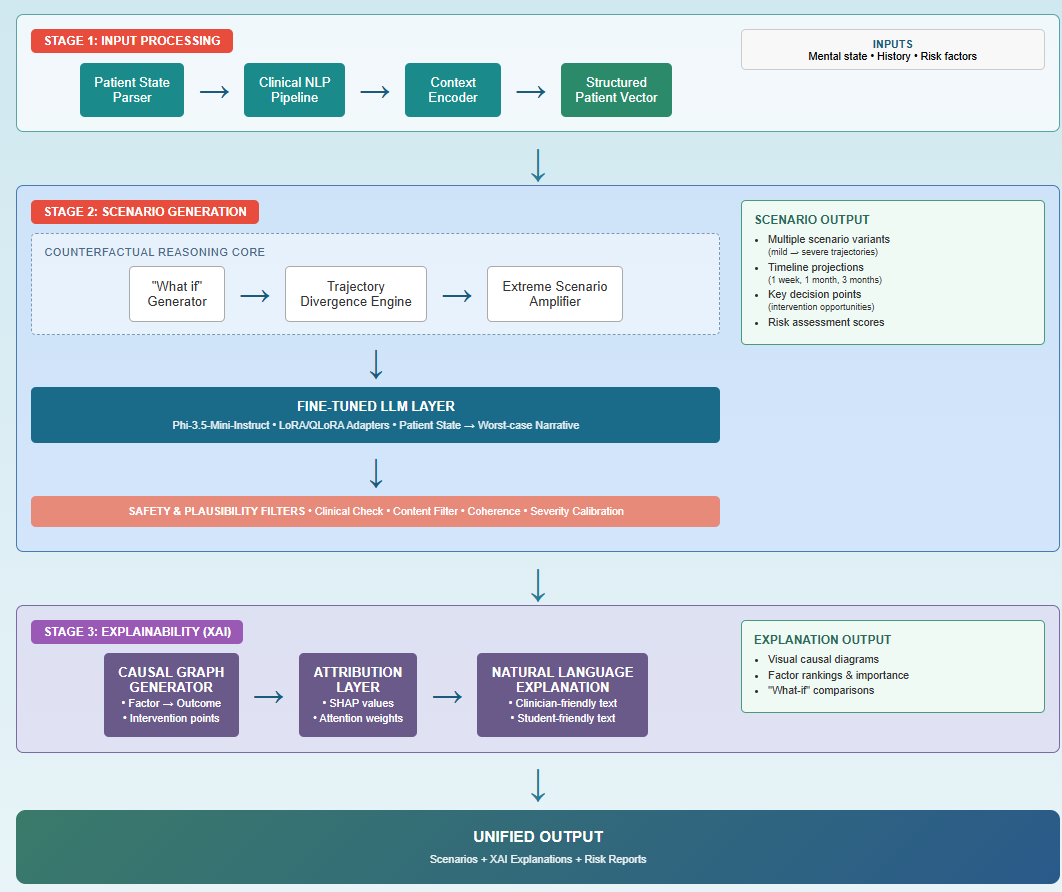
\includegraphics[width=\columnwidth]{images/Flow_diagram.png}
\caption{System architecture of the proposed Mental Health Scenario Processing Engine. Stage~1 extracts structured clinical factors from unstructured notes. Stage~2 generates counterfactual extreme scenarios via Tree-of-Thoughts prompting across three pathways. Stage~3 synthesizes a clinical preparedness report.}
\label{fig:architecture}
\end{figure}

\subsection{Stage 1: Clinical Factor Extraction}

The first stage transforms unstructured discharge summaries into structured patient representations anchored to established clinical taxonomies.

\subsubsection{Model Architecture}
We employ Microsoft Phi-3.5-Mini-Instruct as the base LLM, a 3.8B parameter model supporting a 128K token context window. Parameter-efficient fine-tuning is performed using Low-Rank Adaptation (LoRA) \cite{b19} with the following configuration: rank $r = 32$, scaling factor $\alpha = 64$, dropout rate 0.05, applied to the query, key, value, output, gate, up, and down projection matrices. This adapts 50.3 million parameters (1.30\% of total) while preserving pre-trained capabilities.

\subsubsection{Extraction Schema}
The extraction follows a clinically curated DSM-5 and ICD-11 grounded schema comprising 14 structured fields across 6 categories:

\textbf{Diagnostic Information:}
\begin{itemize}
\item Primary mental health diagnosis (ICD code, title, DSM-5 category)
\item Comorbid mental health diagnoses (array)
\item Medical comorbidities (top 5 by priority)
\item Overall severity level (mild/moderate/severe/critical)
\end{itemize}

\textbf{Suicide Risk Indicators:}
\begin{itemize}
\item Ideation mentioned (boolean)
\item Attempt history (boolean)
\item Self-harm (boolean)
\item Precautions ordered (boolean)
\end{itemize}

\textbf{Substance Use Profile:}
\begin{itemize}
\item Alcohol use (none/use/abuse/dependence)
\item Drug use status
\item Toxicology screen results
\end{itemize}

\textbf{Medication and Treatment:}
\begin{itemize}
\item Psychotropic medications with drug class
\item Polypharmacy indicator
\item Medication count
\end{itemize}

\textbf{Social Factors:}
\begin{itemize}
\item Marital status, insurance type
\item Social isolation risk indicator
\end{itemize}

\textbf{Admission Context:}
\begin{itemize}
\item Admission type, emergency status
\item Length of stay, discharge disposition
\end{itemize}

\subsubsection{Prompt Format}
The extraction prompt follows a structured format aligned between training and inference:

\begin{verbatim}
<|system|>
You are a clinical AI assistant 
specialized in mental health. Extract 
structured clinical factors from the 
patient note according to the schema.
Output valid JSON only.<|end|>
<|user|>
### Clinical Note:
{note_text}
### Extraction Schema:
{schema_json}
### Instructions:
Extract all relevant clinical factors.
Return a JSON object matching the schema.
<|end|>
<|assistant|>
\end{verbatim}

Clinical notes are truncated to 6,000 characters to match training constraints while preserving the most clinically relevant sections.

\subsection{Stage 2: Extreme Scenario Generation}

The second stage employs Tree-of-Thoughts (ToT) prompting to generate counterfactual narratives of extreme adverse mental health trajectories.

\subsubsection{Three-Branch Architecture}
Scenario generation is structured across three clinically distinct escalation pathways, each explored independently:

\textbf{Branch A -- Psychiatric/Clinical Deterioration:} Focuses on how the patient's primary psychiatric condition could worsen through medication non-adherence, treatment resistance, relapse, acute decompensation, re-hospitalization, emergence of psychosis, or escalating self-harm.

\textbf{Branch B -- Substance Use Escalation:} Focuses on how the patient could develop or worsen substance use (alcohol, opioids, stimulants) as a coping mechanism or due to untreated distress, leading to comorbid substance use disorder, impaired judgment, or overdose risk.

\textbf{Branch C -- Social/Environmental Collapse:} Focuses on how the patient's social safety net could erode through housing instability, relationship breakdown, unemployment, or social isolation, removing protective factors and accelerating crisis without a recovery anchor.

\subsubsection{Three-Step ToT Process}
For each branch, three deliberate reasoning steps are executed:

\textbf{Step 1 (Identify):} Identify 3--5 factors already present in the patient's extracted data that could trigger this specific pathway. Each factor is assessed for mental health relevance (high/medium/low).

\textbf{Step 2 (Reason):} Trace a 4--6 step causal chain from triggering factors to a clinical crisis endpoint, specifying the biological, psychological, or social mechanism at each step.

\textbf{Step 3 (Narrate):} Generate a structured scenario analysis comprising:
\begin{itemize}
\item Narrative (2--3 paragraphs in clinical language)
\item Warning signs (3--5 indicators clinicians should monitor)
\item Crisis endpoint (worst realistic outcome)
\item Preparedness actions (3--5 concrete interventions)
\item Plausibility rating with rationale
\item Mental health relevance rating
\end{itemize}

\subsubsection{Mental Health Relevance Filter}
A critical safety feature addresses patients whose primary condition is non-psychiatric (e.g., cardiac surgery, respiratory illness). Before scenario generation, the model assesses whether the patient has significant psychiatric history and rates overall mental health scenario relevance. For patients with low mental health relevance, the model is instructed to:
\begin{itemize}
\item Acknowledge that the primary medical condition does not directly cause psychiatric deterioration
\item Identify only genuine, evidence-based psychiatric consequences (adjustment disorder, post-surgical depression, medication-induced mood changes)
\item Rate scenarios as LOW plausibility when minimal mental health basis exists
\item Avoid fabricating psychotic episodes or suicidal ideation for patients with no psychiatric history
\end{itemize}

\subsection{Stage 3: Clinical Report Generation}

The third stage synthesizes extracted factors and generated scenarios into a structured clinical preparedness report designed as a ``second reader'' briefing.

\subsubsection{Report Structure}
The generated report comprises:
\begin{itemize}
\item \textbf{Patient Overview:} Demographics, primary diagnosis, admission reason, key clinical features
\item \textbf{Mental Health Status:} Current psychiatric state and implications
\item \textbf{Key Risk Factors:} Prioritized list from extracted data
\item \textbf{Protective Factors:} Factors that reduce risk
\item \textbf{Scenario Briefing:} Summary of each pathway with plausibility and key concerns
\item \textbf{Priority Actions:} Top 5 actionable clinical recommendations
\item \textbf{Risk Tier:} Overall rating (HIGH/MODERATE/LOW) with justification
\end{itemize}

\subsubsection{Design Philosophy}
The report is designed as an augmentation tool rather than an autonomous decision-maker. By presenting extreme boundary scenarios with identified intervention points, it enables clinicians to mentally rehearse worst-case trajectories and identify preparedness actions that might not be immediately apparent from the original note alone.

\section{Experimental Setup}

\subsection{Dataset}

The framework is developed using the MIMIC-IV (v3.1) clinical database \cite{b14}, a publicly available de-identified electronic health record dataset from the Beth Israel Deaconess Medical Center containing records spanning 2008--2022.

\subsubsection{Cohort Selection}
The mental health cohort is constructed by filtering admissions using ICD-9 codes 290--319 (mental disorders) and ICD-10 codes F01--F99 (mental, behavioral, and neurodevelopmental disorders). Discharge summaries are extracted from the MIMIC-IV Note module and linked via subject and admission identifiers.

\subsubsection{Dataset Statistics}
Table~\ref{tab:dataset} presents the final dataset composition after filtering and processing.

\begin{table}[t]
\caption{Dataset Composition}
\label{tab:dataset}
\centering
\begin{tabular}{lcc}
\hline
\textbf{Split} & \textbf{Patients} & \textbf{Examples} \\
\hline
Training & 45,223 & 94,592 \\
Validation & 5,640 & 11,409 \\
Test & 5,640 & 11,916 \\
\hline
\textbf{Total} & \textbf{56,503} & \textbf{117,917} \\
\hline
\end{tabular}
\end{table}

The dataset is stratified by primary DSM-5 category and mortality outcome. Table~\ref{tab:stratification} shows the distribution across diagnostic categories.

\begin{table}[t]
\caption{Stratification by DSM-5 Category}
\label{tab:stratification}
\centering
\begin{tabular}{lc}
\hline
\textbf{DSM-5 Category} & \textbf{Examples} \\
\hline
Depressive Disorders & 37,616 \\
Anxiety Disorders & 23,607 \\
Substance Use Disorders & 22,947 \\
Neurocognitive Disorders & 16,472 \\
Bipolar Disorders & 6,175 \\
Schizophrenia/Psychotic & 4,386 \\
Other Mental Health & 3,414 \\
Trauma/Stress Disorders & 2,185 \\
Neurodevelopmental & 619 \\
Personality Disorders & 443 \\
Somatic Disorders & 53 \\
\hline
\end{tabular}
\end{table}

\subsubsection{Label Construction}
Training labels (silver labels) are constructed programmatically by joining structured MIMIC-IV tables:
\begin{itemize}
\item Diagnoses from \texttt{diagnoses\_icd} with ICD-to-DSM-5 mapping
\item Severity derived from DRG codes, ICU flags, and acuity scores
\item Suicide risk indicators from ICD codes for self-harm (E950--E959, X71--X83, T14.91)
\item Substance use from diagnosis codes and toxicology results
\item Medications from \texttt{prescriptions} table filtered to psychotropic drug classes
\item Social factors from \texttt{admissions} (marital status, insurance)
\end{itemize}

\subsection{Training Configuration}

\subsubsection{Hardware}
Training is conducted on a DGX system with 6 NVIDIA Tesla V100-SXM2-32GB GPUs (204.6 GB total GPU memory).

\subsubsection{Hyperparameters}
Table~\ref{tab:hyperparams} presents the training configuration.

\begin{table}[t]
\caption{Training Hyperparameters}
\label{tab:hyperparams}
\centering
\begin{tabular}{ll}
\hline
\textbf{Parameter} & \textbf{Value} \\
\hline
Base Model & microsoft/Phi-3.5-mini-instruct \\
Total Parameters & 3,871,411,200 \\
Trainable Parameters & 50,331,648 (1.30\%) \\
LoRA Rank ($r$) & 32 \\
LoRA Alpha ($\alpha$) & 64 \\
LoRA Dropout & 0.05 \\
LoRA Targets & q, k, v, o, gate, up, down \\
Learning Rate & $2 \times 10^{-4}$ \\
Warmup Ratio & 0.03 \\
LR Schedule & Cosine decay \\
Per-Device Batch Size & 2 \\
Gradient Accumulation & 8 steps \\
Effective Batch Size & 64--96 \\
Number of Epochs & 5 \\
Max Sequence Length & 2,048 tokens \\
Precision & FP16 mixed precision \\
\hline
\end{tabular}
\end{table}

\subsubsection{Training Infrastructure}
Training utilizes the Hugging Face PEFT, TRL, and Transformers libraries with DeepSpeed ZeRO-2 optimization for multi-GPU distribution. Experiment tracking is performed via ClearML.

\section{Results and Analysis}

\subsection{Training Convergence}

Table~\ref{tab:training_results} presents the key training metrics recorded via ClearML.

\begin{table}[t]
\caption{Training Results Summary}
\label{tab:training_results}
\centering
\begin{tabular}{ll}
\hline
\textbf{Metric} & \textbf{Value} \\
\hline
Total Training Time & 35.8 hours \\
Total Training Steps & 7,390 \\
Initial Training Loss & 11.96 \\
Final Training Loss & 1.67 \\
Initial Eval Loss & 4.08 \\
Best Eval Loss & 1.706 \\
Final Perplexity & 5.51 \\
Initial Token Accuracy & 0.0\% \\
Final Token Accuracy & 67.5\% \\
Total FLOPs & $1.096 \times 10^{19}$ \\
Throughput & 3.67 samples/sec \\
\hline
\end{tabular}
\end{table}

The model demonstrates consistent convergence across all 5 epochs. Evaluation loss decreases from 4.08 (epoch 1) to 1.706 (epoch 5), representing a 58.2\% reduction. Mean token accuracy improves from near-zero to 67.5\%, indicating the model learns to produce structurally correct JSON outputs aligned with the extraction schema.

\subsection{Loss Curve Analysis}

Fig.~\ref{fig:loss} shows the training and evaluation loss curves across training steps. The training loss exhibits rapid initial decrease followed by gradual convergence, while evaluation loss shows consistent improvement without overfitting, suggesting the model generalizes rather than memorizing training examples.

\begin{figure}[t]
\centering
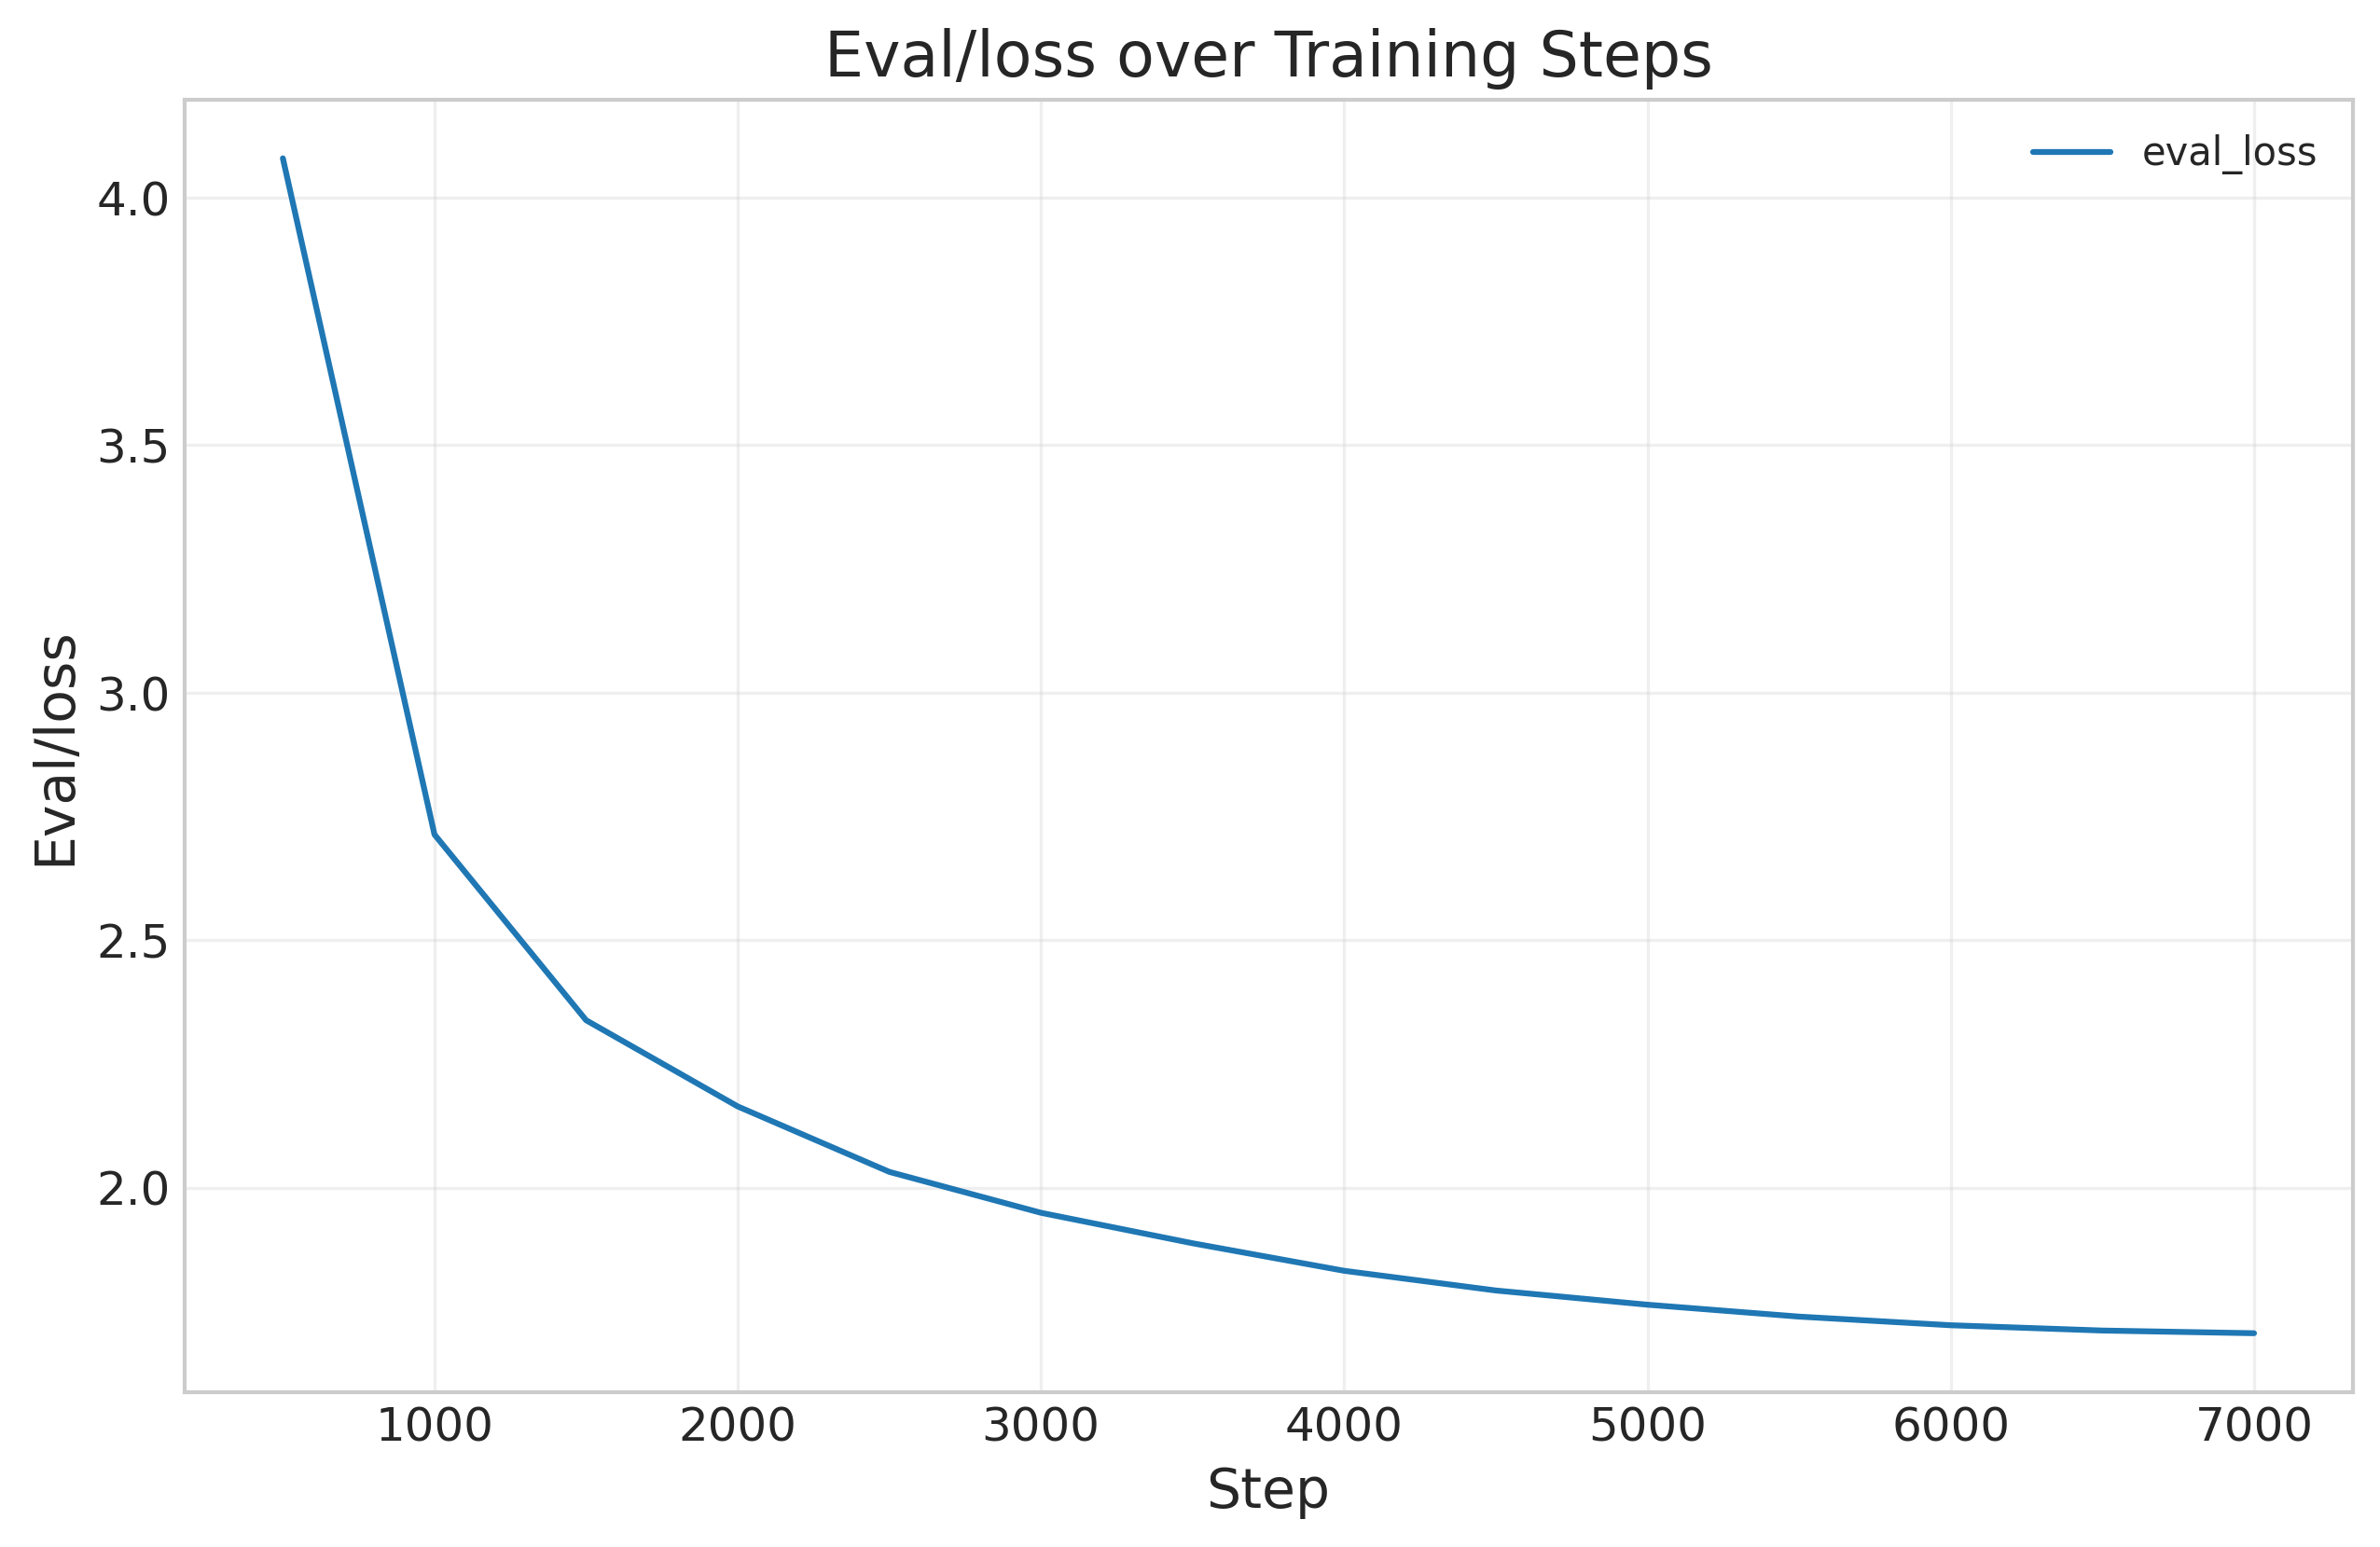
\includegraphics[width=\columnwidth]{images/Eval_loss.png}
\caption{Evaluation loss over training steps, demonstrating consistent convergence from 4.08 to 1.706 across 5 epochs.}
\label{fig:loss}
\end{figure}

\subsection{Qualitative Analysis of Pipeline Output}

To illustrate the framework's behavior, we present a representative example from the test set.

\subsubsection{Input Note (Excerpt)}
A discharge summary for a patient with bipolar disorder and post-traumatic stress disorder, admitted following medication non-adherence and mood decompensation.

\subsubsection{Stage 1 Output: Extracted Factors}
\begin{verbatim}
{
  "primary_mh_diagnosis": {
    "icd_code": "F319",
    "title": "Bipolar disorder, unspecified",
    "dsm5_category": "bipolar_disorders"
  },
  "comorbid_mh_diagnoses": [
    {"icd_code": "F4310", 
     "title": "PTSD, unspecified"}
  ],
  "severity_level": "moderate",
  "suicide_risk_indicators": {
    "ideation_mentioned": true,
    "attempt_history": false,
    "self_harm": false
  },
  "substance_use": {
    "alcohol": "history",
    "drugs": "none"
  }
}
\end{verbatim}

\subsubsection{Stage 2 Output: Scenario Branch A}
\textbf{Triggering Factors Identified:}
\begin{enumerate}
\item Documented medication non-adherence (high MH relevance)
\item History of mood decompensation requiring hospitalization (high)
\item Comorbid PTSD complicating treatment response (medium)
\end{enumerate}

\textbf{Crisis Endpoint:} Severe manic episode with psychotic features requiring involuntary psychiatric hospitalization.

\textbf{Plausibility:} Medium---patient has documented non-adherence pattern but current stabilization on lithium.

\subsubsection{Stage 3 Output: Report Summary}
\textbf{Risk Tier:} MODERATE

\textbf{Priority Actions:}
\begin{enumerate}
\item Establish medication adherence monitoring protocol
\item Schedule follow-up within 7 days post-discharge
\item Provide crisis hotline information and safety planning
\item Coordinate with outpatient psychiatry for continuity
\item Assess social support availability
\end{enumerate}

\subsection{Observations on Model Behavior}

Analysis of pipeline outputs across multiple test cases reveals several patterns:

\textbf{Strengths:}
\begin{itemize}
\item Consistent JSON structure in extraction (when parsing succeeds)
\item Appropriate grounding to DSM-5 categories
\item Reasonable identification of risk factors from clinical text
\item Plausibility ratings generally correlate with clinical evidence
\end{itemize}

\textbf{Limitations Observed:}
\begin{itemize}
\item Parse failures on approximately 10--15\% of complex notes
\item Occasional hallucination of risk factors not present in source
\item Verbose or repetitive scenario narratives in some cases
\item Difficulty with non-psychiatric patients (medical-only admissions)
\end{itemize}

\section{Discussion}

\subsection{Key Contributions}

This work presents several contributions to mental health clinical NLP:

\textbf{Novel Application:} To our knowledge, this is the first implemented system applying counterfactual scenario generation specifically for mental health clinical preparedness, shifting the paradigm from prediction to preparation.

\textbf{Schema-Grounded Extraction:} The DSM-5/ICD-11 grounded extraction schema provides structured, auditable factor extraction rather than opaque risk scores.

\textbf{Tree-of-Thoughts Prompting:} The three-branch ToT architecture enables systematic exploration of distinct escalation pathways, avoiding the limitations of single-trajectory generation.

\textbf{Reproducible Training:} Complete training configuration and convergence analysis on a publicly available dataset (MIMIC-IV) supports reproducibility.

\subsection{Limitations}

Several significant limitations must be acknowledged:

\textbf{No Ground Truth Evaluation:} This work presents training metrics (loss, perplexity, token accuracy) but does not include evaluation against manually annotated ground truth labels. Future work must establish gold-standard annotations to compute precision, recall, and F1 scores for extraction quality.

\textbf{No Downstream Task Evaluation:} We do not evaluate whether the extracted factors or generated scenarios improve clinical decision-making. Metrics such as classification AUROC for risk prediction remain unmeasured.

\textbf{No Clinician Validation:} Generated scenarios have not been evaluated by clinical experts for plausibility, clinical accuracy, or utility. Clinician evaluation studies are essential for deployment validation.

\textbf{Hallucination Risk:} Like all generative models, the system can fabricate clinical details not present in source notes. Hallucination rate has not been formally quantified.

\textbf{Dataset Bias:} MIMIC-IV is ICU-centric; most notes originate from medical/surgical ICU stays where mental health conditions are secondary. Performance on dedicated psychiatric unit notes may differ.

\textbf{No Explainability Module:} While the original design envisioned a causal explainability layer with SHAP values and attention analysis, this module is not implemented in the current system. Generated explanations are purely text-based without computational attribution.

\subsection{Ethical Considerations}

Deployment of AI systems for mental health requires careful ethical consideration:

\begin{itemize}
\item The system is designed as a ``second reader'' augmentation tool, not a replacement for clinical judgment
\item All training data is de-identified per HIPAA requirements
\item Generated extreme scenarios could cause distress if presented inappropriately; output filtering and clinical context framing are essential
\item The system should not be used for autonomous clinical decisions
\end{itemize}

\section{Conclusion and Future Work}

This paper presented the design, implementation, and training of a fine-tuned LLM framework for counterfactual simulation of extreme mental health scenarios. The system employs a LoRA-adapted Microsoft Phi-3.5-Mini-Instruct model trained on 94,592 MIMIC-IV discharge summaries, achieving evaluation loss of 1.706 and 67.5\% mean token accuracy for structured clinical factor extraction. A Tree-of-Thoughts prompting architecture enables generation of counterfactual scenarios across three distinct escalation pathways.

The framework represents a methodological contribution to clinical NLP, demonstrating the feasibility of counterfactual preparedness systems for mental health. However, significant work remains before clinical deployment:

\textbf{Future Work:}
\begin{enumerate}
\item \textbf{Gold-standard annotation:} Manual annotation of 200+ test notes to enable quantitative extraction evaluation
\item \textbf{Clinician evaluation:} Structured review of generated scenarios by mental health professionals
\item \textbf{Hallucination quantification:} Formal measurement of factual accuracy against source notes
\item \textbf{Downstream task evaluation:} Assessment of whether the framework improves clinical outcomes or decision quality
\item \textbf{Explainability module:} Implementation of attention-based attribution and causal pathway visualization
\item \textbf{Multi-center validation:} Evaluation on datasets from dedicated psychiatric facilities
\end{enumerate}

The code and trained model adapters will be made available upon publication to support reproducibility and further research.

\section*{Acknowledgment}

The authors acknowledge the use of the MIMIC-IV dataset, made available by the MIT Laboratory for Computational Physiology through PhysioNet.

\begin{thebibliography}{00}

\bibitem{b1} GBD 2019 Mental Disorders Collaborators, ``Global, regional, and national burden of 12 mental disorders in 204 countries and territories, 1990--2019: A systematic analysis for the Global Burden of Disease Study 2019,'' \textit{The Lancet Psychiatry}, vol. 9, no. 2, pp. 137--150, Feb. 2022.

\bibitem{b2} B. G. Teferra, S. Langan, and S. Rose, ``NLP for mental health interventions: A systematic review and research framework,'' \textit{Translational Psychiatry}, vol. 13, no. 1, p. 309, Oct. 2023.

\bibitem{b3} E. Sezgin, S.-A. Hussain, S. Rust, and Y. Huang, ``Extracting medical information from free-text and unstructured patient-generated health data using natural language processing methods: Feasibility study with real-world data,'' \textit{JMIR Formative Research}, vol. 7, p. e43014, Jan. 2023.

\bibitem{b4} X. Xu et al., ``Mental-LLM: Leveraging large language models for mental health prediction via online text data,'' \textit{Proc. ACM Interactive Mobile Wearable Ubiquitous Technol.}, vol. 8, no. 1, pp. 1--32, Mar. 2024.

\bibitem{b5} Z. Guo, A. Lai, J. H. Thygesen, J. Farrington, T. Keen, and K. Li, ``Large language models for mental health applications: Systematic review,'' \textit{JMIR Mental Health}, vol. 11, p. e57400, Sep. 2024.

\bibitem{b6} Y. Hua et al., ``Large language models in mental health care: A scoping review,'' \textit{arXiv preprint}, arXiv:2401.02984, Jan. 2024.

\bibitem{b7} A. M. Alkalbani et al., ``A systematic review of large language models in medical specialties: Applications, challenges and future directions,'' \textit{Information}, vol. 16, no. 6, p. 489, Jun. 2025.

\bibitem{b8} M. Prosperi et al., ``The clinical potential of counterfactual AI models,'' \textit{The Lancet}, vol. 403, no. 10432, pp. 1063--1065, Mar. 2024.

\bibitem{b9} I. Gat et al., ``Counterfactual modeling with fine-tuned large language models,'' \textit{arXiv preprint}, arXiv:2601.14590, Jan. 2026.

\bibitem{b14} A. Johnson et al., ``MIMIC-IV, a freely accessible electronic health record dataset,'' \textit{Scientific Data}, vol. 10, no. 1, p. 1, Jan. 2023.

\bibitem{b15} B. G. Teferra et al., ``Screening for depression using natural language processing: Literature review,'' \textit{Interactive Journal of Medical Research}, vol. 13, p. e55067, Nov. 2024.

\bibitem{b16} S. K. Lho et al., ``Large language models and text embeddings for detecting depression and suicide in patient narratives,'' \textit{JAMA Network Open}, vol. 8, no. 5, p. e2511922, May 2025.

\bibitem{b17} W. Kim and C. Wang, ``Large language models for interpretable mental health diagnosis with DSM-5 grounding,'' in \textit{Proc. LLM4Health Workshop}, 2025.

\bibitem{b18} Y. Chen, L. Zhong, and N. F. Rajani, ``Do models explain themselves? Counterfactual simulatability of natural language explanations,'' \textit{arXiv preprint}, arXiv:2307.08678, Jul. 2023.

\bibitem{b19} E. J. Hu et al., ``LoRA: Low-rank adaptation of large language models,'' in \textit{Proc. Int. Conf. Learning Representations (ICLR)}, 2022.

\end{thebibliography}

\end{document}
